\section{预算分配}
\label{sec:budget-allocation}

有了成本账，下一个问题是同一笔预算怎样分。几乎每种改进都要求先花一部分计算去“了解问题”：重要性采样要先拟合建议分布，控制变量要先估计系数，分层要先知道各层的波动，Markov链要先跑掉初值的影响。花得太少，方案选得差；花得太多，留给正式计算的就少了。成组随机化还有另一种分法：总点数一定时，每组放多少点、重复多少组。

\paragraph{试运行与正式计算}
设总预算为$C$。先用$n_{0}$个试运行样本（每个成本$c_{0}$）确定方法的参数$\hat{\lambda}$，再用剩下的预算按$\hat{\lambda}$做正式计算，每个正式样本成本为$c$。正式计算使用与试运行独立的新随机数，所以在给定试运行结果的条件下，正式估计仍是无偏的独立样本平均（第~\ref{chap:variance-reduction}章对固定建议后的估计证明了这一点），其条件方差为$v(\hat{\lambda})c/(C-n_{0}c_{0})$，这里$v(\lambda)$是参数取$\lambda$时的单样本方差。对试运行取期望，最终估计的方差是
\begin{equation}
  \operatorname{Var}(\hat{I})=\frac{\mathbb{E}\bigl[v(\hat{\lambda})\bigr]\,c}{C-n_{0}c_{0}} .
  \label{eq:budget-pilot-var}
\end{equation}
分子随$n_{0}$增大而减小，因为参数估得更准；分母也随$n_{0}$增大而减小，因为正式计算的预算变少。

为看清两种作用怎样平衡，设$\hat{\lambda}$随$n_{0}\to\infty$收敛到$\bar{\lambda}$，$v$在$\bar{\lambda}$附近光滑，且$\hat{\lambda}-\bar{\lambda}$的均方按$1/n_{0}$缩小。

若$\bar{\lambda}$是$v$的最小点，展开到二阶，一阶项消失；若不是，$\hat{\lambda}$的偏差与波动也只在$1/n_{0}$阶贡献额外方差。两种情形都可以写成
\[
  \mathbb{E}\bigl[v(\hat{\lambda})\bigr]\approx\bar{v}+\frac{a}{n_{0}},
\]
其中$\bar{v}=v(\bar{\lambda})$，$a>0$概括参数估计误差的影响。代入式~\eqref{eq:budget-pilot-var}，要最小化
\[
  g(n_{0})=\frac{\bar{v}+a/n_{0}}{C-n_{0}c_{0}} .
\]
令$g'(n_{0})=0$，即
\[
  -\frac{a}{n_{0}^{2}}\,(C-n_{0}c_{0})+c_{0}\Bigl(\bar{v}+\frac{a}{n_{0}}\Bigr)=0,
\]
两边乘以$n_{0}^{2}$并整理，得到
\[
  c_{0}\bar{v}\,n_{0}^{2}+2ac_{0}\,n_{0}-aC=0 .
\]
取正根，并在$C$远大于$ac_{0}/\bar{v}$时保留主项，得到
\begin{equation}
  n_{0}^{\ast}\approx\sqrt{\frac{aC}{c_{0}\bar{v}}},\qquad\frac{n_{0}^{\ast}c_{0}}{C}\approx\sqrt{\frac{ac_{0}}{\bar{v}C}} .
  \label{eq:budget-pilot-opt}
\end{equation}
试运行的样本数按$\sqrt{C}$增长，占总预算的比例按$1/\sqrt{C}$缩小。预算越大，越值得把参数估准，但越不必为此花上一个固定的比例。

用本章开头的尾概率演示。试运行从覆盖尾部的$q_{0}=\operatorname{Exp}(1/2)$抽样，每个样本对积分的贡献为$c_{i}=\mathbf{1}_{\{Y_i>4\}}p(Y_i)/q_{0}(Y_i)$。第~\ref{chap:variance-reduction}章说明理想的建议分布正比于$\mathbf{1}_{\{x>4\}}\mathrm{e}^{-x}$，其均值为$5$。在指数族$\operatorname{Exp}(\lambda)$中，用贡献加权的均值去匹配$1/\lambda$：
\[
  \hat{\lambda}=\frac{\sum_{i}c_i}{\sum_{i}c_iY_i},
\]
试运行没有样本超过$4$时保留$\lambda=1/2$。$n_{0}\to\infty$时$\hat{\lambda}\to1/5$，此时单样本方差$v(0.2)\approx0.001738$，与族内最优$\lambda^{\ast}\approx0.219$处的$v^{\ast}\approx0.001730$只差$0.5\%$。试运行与正式样本的成本都记为$1.5$。

图~\ref{fig:budget-pilot-size}画出三种预算下最终的相对均方根误差$\sqrt{\operatorname{Var}(\hat{I})}/I$随$n_{0}$的变化，条件方差用精确公式计算，对试运行的期望用模拟（种子$7$）。三条曲线的谷底都很平：$C=1500$时最好的$n_{0}$约为$37$，相对均方根误差约$0.074$，比已知最优建议分布的$0.072$只差一点；$n_{0}$小到$5$时误差约$0.084$，只高出约$14\%$；$n_{0}$大到预算的$70\%$时误差约$0.131$，高出约$78\%$。作为对照，同样预算的直接平均相对误差约为$0.19$。三种预算的最优$n_{0}$随$C$右移，但远慢于$C$本身的增长，与式~\eqref{eq:budget-pilot-opt}一致。

\begin{BookInlineFigure}
  \centering
  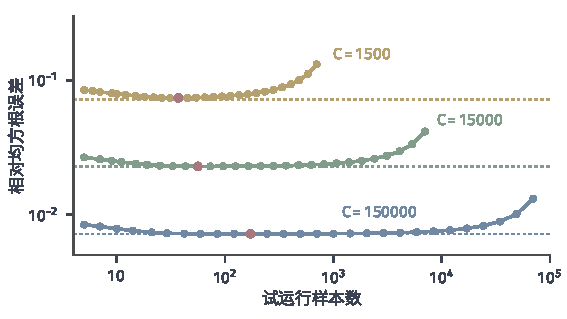
\includegraphics[width=96mm]{figures/07-probability/08-sampling-and-integration/matplotlib/budget-pilot-size/figure.pdf}
  \caption{试运行规模与最终精度。目标$I=\mathbb{P}(X>4)$，$X\sim\operatorname{Exp}(1)$；试运行从$\operatorname{Exp}(1/2)$抽取$n_{0}$个样本拟合$\lambda$，正式计算用新随机数从$\operatorname{Exp}(\hat{\lambda})$抽样，每个样本成本$1.5$。三条曲线对应总预算$C=1500$、$15000$、$150000$，点线为已知最优$\lambda^{\ast}$时的误差，红点为各曲线的最小点。}
  \label{fig:budget-pilot-size}
\end{BookInlineFigure}

这个例子的拟合问题很容易，只有一个参数，所以谷底特别平。参数多、贡献区域分散时，$a$会大得多，过小的试运行可能根本没有观察到某个贡献区域，这时式~\eqref{eq:budget-pilot-opt}所依据的“误差按$1/n_{0}$缩小”还没有开始成立。第~\ref{sec:budget-stopping}节讨论这种情形。

\paragraph{预备开销的分摊}
控制变量的系数也可以由试运行估计。用$n_{0}$个独立的试运行样本估计$\hat{\beta}$，再用新样本计算$f-\hat{\beta}(h-\mathbb{E}h)$的平均，给定$\hat{\beta}$时正式估计无偏，方差为$\operatorname{Var}\bigl(f-\hat{\beta}h\bigr)/n$，分析与式~\eqref{eq:budget-pilot-var}相同。若用同一批样本既估系数又求平均，省下了试运行，却引入$1/n$阶的有限样本偏差（第~\ref{chap:variance-reduction}章），预算较大时这一偏差相对于波动可以忽略，预算很小时则要计入。

分层采样把预备开销与分配规则联系在一起。设$K$层的概率为$p_k$，层内单样本方差为$\sigma_k^{2}$，层内每个样本的成本为$c_k$，第$k$层抽$n_k$个样本。

分层估计的方差与总成本分别是
\[
  \sum_{k=1}^{K}\frac{p_k^{2}\sigma_k^{2}}{n_k},\qquad\sum_{k=1}^{K}n_kc_k=C .
\]
由Cauchy--Schwarz不等式，
\[
  \Bigl(\sum_{k}p_k\sigma_k\sqrt{c_k}\Bigr)^{2}=\Bigl(\sum_{k}\frac{p_k\sigma_k}{\sqrt{n_k}}\cdot\sqrt{n_kc_k}\Bigr)^{2}\le\sum_{k}\frac{p_k^{2}\sigma_k^{2}}{n_k}\cdot\sum_{k}n_kc_k,
\]
等号当且仅当$\sqrt{n_kc_k}$与$p_k\sigma_k/\sqrt{n_k}$成比例。于是固定预算下的最优分配与最小方差为
\begin{equation}
  n_k\propto\frac{p_k\sigma_k}{\sqrt{c_k}},\qquad\operatorname{Var}_{\min}=\frac{1}{C}\Bigl(\sum_{k=1}^{K}p_k\sigma_k\sqrt{c_k}\Bigr)^{2} .
  \label{eq:budget-neyman-cost}
\end{equation}

式~\eqref{eq:budget-neyman-cost}要求知道各层的$\sigma_k$和$c_k$，实际只能由试运行估计，而估计的成本与估计误差都要计入。按$n_k\propto p_k$的比例分配不需要这些信息，在样本总数相同时其方差不超过直接平均；把预算从比例分配转向式~\eqref{eq:budget-neyman-cost}，只有在试运行能可靠区分各层波动时才值得。

以$\mathrm{e}^{U}$的$4$层等概率分层为例，各层成本相同，层内标准差依次约为$0.082$、$0.105$、$0.135$、$0.173$。比例分配与式~\eqref{eq:budget-neyman-cost}的最优分配按每个样本折算的方差分别为
\[
  \sum_{k}p_k\sigma_k^{2}\approx0.01653,\qquad\Bigl(\sum_{k}p_k\sigma_k\Bigr)^{2}\approx0.01536,
\]
最优分配把样本按约$0.17:0.21:0.27:0.35$分给四层，只多省约$7\%$。若为估计$\sigma_k$专门做一轮试运行，这点收益很容易被试运行的成本和$\sigma_k$的估计误差抵消；直接平均的$0.2420$到比例分层的$0.0165$才是主要的改进。

\paragraph{多次启动与单链延长}
Markov链的预算$B$（总迭代步数）可以给一条长链，也可以分给$m$条短链，每条$B/m$步，各自舍弃前$b$步。用式~\eqref{eq:budget-ar1}中$\rho=0.9$的自回归链计算，目标$\mathcal{N}(0,1)$，$f(x)=x$，$I=0$，所有链都从$x_{0}=10$启动。这条链的矩可以精确写出：
\[
  \mathbb{E}\bigl[X^{(t)}\bigr]=0.9^{t}x_{0},\qquad\operatorname{Cov}\bigl(X^{(s)},X^{(t)}\bigr)=0.9^{\lvert t-s\rvert}\bigl(1-0.81^{\min(s,t)}\bigr),
\]
于是每种分法的均方误差都可以精确计算。

图~\ref{fig:budget-chain-count}给出$B=2000$时的结果。不舍弃初值（$b=0$）时，一条链的均方误差约$0.0115$，其中偏差约$0.045$；分成$10$条链后偏差升到约$0.45$，均方误差约$0.21$。原因是每条链都带着同样的初值偏差，平均多条链不能抵消它，而每条链越短，初值那一段所占的比例越大。舍弃$b=30$步后，一条链的均方误差约$0.0096$，接近平稳时的$\sigma_{\mathrm{LR}}^{2}/B=19/2000=0.0095$；链数增多，$mb$步的初始化成本吃掉越来越多的预算，$m=50$时均方误差升到约$0.076$。对单峰、链混合良好的目标，只看均方误差，一条长链最省。

单链时舍弃多少步也可以由均方误差估算。设舍弃$b$步后保留$L=B-b$步，初值偏差在平均中留下的部分约为
\[
  \frac{x_{0}}{L}\sum_{t=b+1}^{B}\rho^{t}\approx\frac{x_{0}\rho^{b+1}}{(1-\rho)L},
\]
波动约为$\sigma_{\mathrm{LR}}^{2}/L$。$b$每增加$1$，偏差平方约乘以$\rho^{2}$，减少量约为偏差平方的$2\ln(1/\rho)$倍；波动则因$L$减少$1$而约增加$\sigma_{\mathrm{LR}}^{2}/L^{2}$。在最优的$b$处二者相等，
\[
  2\ln\frac1\rho\cdot\frac{x_{0}^{2}\rho^{2b+2}}{(1-\rho)^{2}L^{2}}=\frac{\sigma_{\mathrm{LR}}^{2}}{L^{2}},
  \qquad\text{即}\qquad
  \rho^{2b+2}=\frac{\sigma_{\mathrm{LR}}^{2}(1-\rho)^{2}}{2x_{0}^{2}\ln(1/\rho)} .
\]
代入$\rho=0.9$、$x_{0}=10$、$\sigma_{\mathrm{LR}}^{2}=19$，右边约为$0.0090$，解得$b\approx21$，与精确计算的最优值$21$一致。舍弃步数只按$\ln x_{0}$增长：初值离目标越远，舍弃越多，但远小于总预算。这个估算要求知道链向目标靠拢的速度$\rho$，一般的链只能由试运行或理论估计。

\begin{BookInlineFigure}
  \centering
  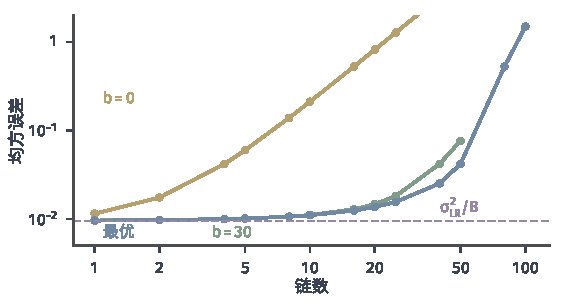
\includegraphics[width=96mm]{figures/07-probability/08-sampling-and-integration/matplotlib/budget-chain-count/figure.pdf}
  \caption{总预算$B=2000$步分给$m$条链时的精确均方误差。自回归链系数$0.9$，目标$\mathcal{N}(0,1)$，$f(x)=x$，每条链从$x_{0}=10$启动并舍弃前$b$步。黄线$b=0$，绿线$b=30$，蓝线对每个$m$取最优$b$；紫色虚线为平稳单链的$\sigma_{\mathrm{LR}}^{2}/B$。}
  \label{fig:budget-chain-count}
\end{BookInlineFigure}

多次启动的价值在别处：它是发现链没有走遍目标的少数手段之一。图~\ref{fig:budget-multistart}在双峰混合$0.3\,\mathcal{N}(-2,0.5^{2})+0.7\,\mathcal{N}(2,1)$上用步长$s=0.5$的随机游走Metropolis，从$-4,-1,1,4$四个分散的初值各跑$500$步。从$-4$与$-1$出发的两条链始终留在左峰，平均约$-2.0$；从$4$出发的一条始终在右峰，平均约$2.15$；从$1$出发的一条在第$270$步左右才跨到左峰。只看任何一条链，运行均值都会在某个错误的值附近“稳定”下来。

\begin{BookInlineFigure}
  \centering
  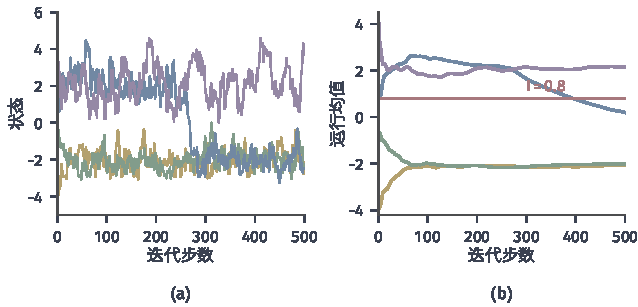
\includegraphics[width=108mm]{figures/07-probability/08-sampling-and-integration/matplotlib/budget-multistart/figure.pdf}
  \caption{双峰混合$0.3\,\mathcal{N}(-2,0.5^{2})+0.7\,\mathcal{N}(2,1)$上的随机游走Metropolis（步长$0.5$），四条链分别从$-4$（黄）、$-1$（绿）、$1$（蓝）、$4$（紫）启动，种子$0$到$3$。(a)~状态轨迹。(b)~$f(x)=x$的运行均值，红线为$I=0.8$。}
  \label{fig:budget-multistart}
\end{BookInlineFigure}

四条链之间的差异立刻暴露了问题，但把它们合起来平均并不能修正：合并均值约$-0.43$，因为四条链在两个峰上的时间比例反映的是初值的安排，而不是两个峰的概率$0.3$与$0.7$。所以多条链的分歧只能说明“当前的转移核在这个预算内不够用”，补救要回到转移核本身，例如加大步长（图~\ref{fig:budget-sampler-costs}中$s=4$的$\tau_{f}$约为$6.5$）。在预算分配上，这意味着要在单链延长带来的较小相关误差与多次启动带来的探索检查之间取舍：前者对已经走遍目标的链更经济，后者对可能多峰的目标是必要的保险。

\paragraph{成组采样的组内点数与重复数}
拉丁超立方与随机化准蒙特卡洛一次产生一组相关的点，第~\ref{chap:monte-carlo-integration-error}章说明误差要靠整组的独立重复来估计。设每组$n$个点，重复$R$组，总求值次数$N=nR$，另加点集准备的成本。两个参数的作用不同：$n$决定单组估计$Q$的精度，$R$是估计$\operatorname{Var}(Q)$时的独立观测数。

以随机移位网格$a_k=k/n$计算$\int_{0}^{1}\mathrm{e}^{u}\,\mathrm{d}u$为例。单组估计的方差有精确表达式，对大的$n$约为$(\mathrm{e}-1)^{2}/(12n^{2})$（第~\ref{chap:variance-reduction}章）。代入$n=N/R$，$R$组平均的方差为
\[
  \frac{\operatorname{Var}(Q_{n})}{R}\approx\frac{(\mathrm{e}-1)^{2}}{12n^{2}R}=\frac{(\mathrm{e}-1)^{2}R}{12N^{2}} .
\]
总点数固定时，组数越少，平均越准，因为单组方差随$n$下降得比$1/n$快。

可是只有$R$个组估计可用来估计方差，误差区间要用自由度$R-1$的$t$分位数$t_{R-1}$，形如$\bar{Q}\pm t_{R-1}s_{Q}/\sqrt{R}$。$R=2$时$t_{1}\approx12.7$，区间极宽。图~\ref{fig:budget-groups}(a)取$N=1024$，比较平均的均方根误差与区间的平均半宽：均方根误差随$R$单调增大，半宽在$R=4$到$8$附近最小（约$0.003$），$R=2$时约$0.0071$，$R=32$时约$0.0056$。图~\ref{fig:budget-groups}(b)是区间的实际覆盖率：$R=2$与$4$时约$0.93$，低于名义的$0.95$，因为单组估计$Q$的分布接近均匀而非正态；$R\ge8$后接近$0.95$。

\begin{BookInlineFigure}
  \centering
  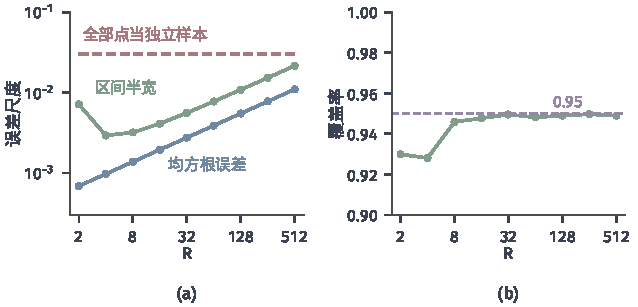
\includegraphics[width=108mm]{figures/07-probability/08-sampling-and-integration/matplotlib/budget-groups/figure.pdf}
  \caption{随机移位网格计算$\int_{0}^{1}\mathrm{e}^{u}\,\mathrm{d}u$，总点数$N=nR=1024$固定，横轴为组数$R$。(a)~蓝线为$R$组平均的均方根误差（精确公式），绿线为区间$\bar{Q}\pm t_{R-1}s_{Q}/\sqrt{R}$的平均半宽，红色虚线为把全部点当作独立样本时的半宽。(b)~该区间的覆盖率，紫色虚线为名义值$0.95$。(a)中的半宽与(b)均由$40000$次模拟得到（种子$3$）。}
  \label{fig:budget-groups}
\end{BookInlineFigure}

图中红色虚线是一个常见的错误：把全部$1024$个点的样本方差除以$1024$，得到半宽约$0.030$，比实际误差大一个数量级以上。这种做法在这里偏于保守，但它说明组内点不是独立样本，其样本方差与组平均的波动无关。对其他点集或被积函数，同样的错误也可能低估误差。综合两张图，总点数一定时，取十几到几十组通常是精度与误差估计可靠性之间的折中；若需要较准确的渐近区间，$R$还应更大，代价是单组的点数减少。
